\section{Sistema di illuminazione}

\begin{figure}[h]
    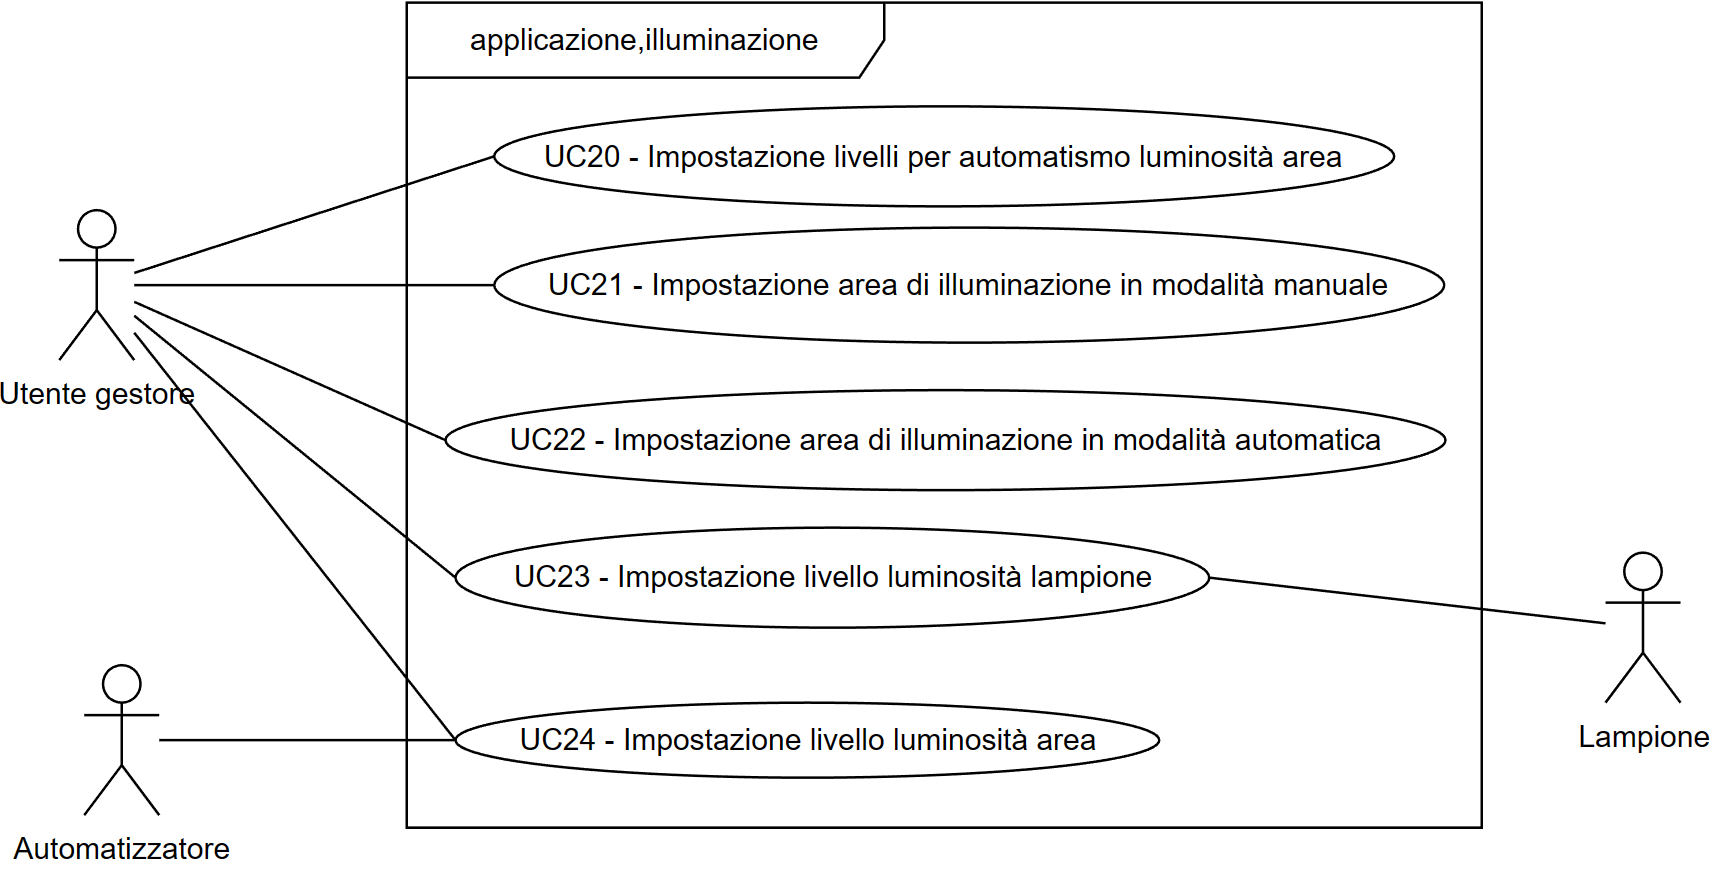
\includegraphics[width=\textwidth]{contenuti/img/casi_uso_grafici-applicazione,illuminazione.png}
    \caption{Parte dell'applicazione relativa alla gestione dell'illuminazione}
    \label{fig:illuminazione}
\end{figure}

\subsection{I casi d'uso descritti}

\begin{itemize}
    \item \hyperref[uc:14]{UC14 - Impostare livelli per automatismo luminositò area}
    \item \hyperref[uc:15]{UC15 - Impostazione area di illuminazione in modalità manuale}
    \item \hyperref[uc:16]{UC16 - Impostare area di illuminazione in modalità automatica}
    \item \hyperref[uc:17]{UC17 - Impostazione livello luminosità lampione}
    \item \hyperref[uc:19]{UC19 - Impostare livello luminosità area}
\end{itemize}
